\newcommand{\mess}[3] {
\begin{figure}[htb]
	\centering
	\includegraphics[width=0.8\textwidth]{#1}
	\caption{#2}
	\label{#3}
\end{figure} }
\newcommand{\refabb}[1]{(siehe Abb. \ref{#1})}

\chapter{Versuchsdurchführung}
\section{Testschaltungen}
\subsection{Verstärkungsfaktor einer nicht-invertierenden Schaltung}
Zur Vorbereitung auf die Benutzung der Operationsverstärker in der Ekg
Schaltung, messen wir Ein- und Ausgangsspannung einer Impedanzwandlerschaltung
und einer nicht-invertierenden Verstärkerschaltung.
\begin{figure}[htb]
    \centering
    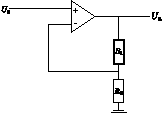
\includegraphics[width=0.6\textwidth]{Abb/nicht-inv.pdf}
    \caption{Schaltung einer nicht-invertierenden Verstärkerschaltung. Die
Verstärkung wird durch das Verhältnis der beiden Widerstände zueinander
bestimmt.}
    \label{ninv}
\end{figure}
Zur Messung benutzen wir ein Signalinterface, um ein Messsignal von
$\SI{0}{\volt}$ bis $\SI{5}{\volt}$ zu generieren und den Output wieder
abzutasten. 
\mess{Mess/Op/faktor1.pdf}{Messung einer Impedanzwandlerschaltung. Die
Verstärkung ist 1. Diese Schaltung wird benutzt um den hohen Widerstand des
Körpers vor der Verstärkung des Ekg Signals zu kompensieren.}{imp}
Zur Messung hoher Verstärkungen benutzen wir einen Spannungsteiler vor dem
Eingang des Verstärkers. In Abbildung \ref{spann} ist das Signal nur durch den
Spannungsteiler zu sehen.
\mess{Mess/Op/spannungsteiler.pdf}{Messung des benutzten Spannungsteiler am
Eingang}{spann}
Zur Messung der nicht-invertierenden Verstärkerschaltung benutzten wir vier
unterschiedliche Widerstandsverhältnisse. 
\begin{center}
\begin{tabular}{c c c}
\hline
$R_1$ &$R_2$ &Verstärkung \\ \hline
$\SI{1}{\kilo \ohm}$ &$\SI{10}{\kilo\ohm}$ &$1.1$ \\
$\SI{33}{\kilo\ohm}$ &$\SI{10}{\kilo\ohm}$ &$4.3$ \\
$\SI{47}{\kilo\ohm}$ &$\SI{10}{\kilo\ohm}$ &$5.7$ \\
$\SI{100}{\kilo\ohm}$ &$\SI{10}{\kilo\ohm}$ &$11$ \\
\hline
\end{tabular}
\end{center}
In \ref{noninv} ist zu erkennen, dass die Verstärkung im Rahmen der Messtoleranz
gut erreicht wurde.
\mess{Mess/Op/noninv.pdf}{Messung der nicht-invertierenden Verstärkerschaltung.
In der Legende sind die Verstärkungen des jeweiligen Aufbaus gelistet. Zur
Messung wurde ein Spannungsteiler am Eingang verwendet, um die maximale Spannung
des AD-Wandlers nicht zu überschreiten.}{noninv}
